\documentclass{article}

\usepackage{fancyhdr} % Required for custom headers
\usepackage{lastpage} % Required to determine the last page for the footer
\usepackage{extramarks} % Required for headers and footers
\usepackage[usenames,dvipsnames]{color} % Required for custom colors
\usepackage{graphicx} % Required to insert images
\usepackage{listings} % Required for insertion of code
\usepackage{courier} % Required for the courier font
\usepackage{lipsum} % Used for inserting dummy 'Lorem ipsum' text into the template
\usepackage{hyperref}
\usepackage{multirow}
\usepackage{tabularx}
\usepackage{longtable}
\usepackage{listings}
\usepackage{subfigure}
\usepackage{afterpage}
\usepackage{amsmath,amssymb}            
\usepackage{rotating}  
\usepackage{fancyhdr}
\usepackage{graphicx}
\usepackage{amsthm}
\usepackage[scriptsize]{caption} 
\hyphenation{a-gen-tiz-za-zio-ne}
% Margins
\topmargin=-0.45in
\evensidemargin=0in
\oddsidemargin=0in
\textwidth=6.5in
\textheight=9.0in
\headsep=0.25in

\linespread{1.1} % Line spacing

\lstset{
  numbers=left,
  stepnumber=5,    
  firstnumber=1,
  numberfirstline=true
}

% Set up the header and footer
\pagestyle{fancy}
\lhead{\hmwkAuthorName} % Top left header
\chead{\hmwkClass\ (\hmwkClassInstructor\ \hmwkClassTime): \hmwkTitle} % Top center head
\rhead{\firstxmark} % Top right header
\lfoot{\lastxmark} % Bottom left footer
\cfoot{} % Bottom center footer
\rfoot{Page\ \thepage\ of\ \protect\pageref{LastPage}} % Bottom right footer
\renewcommand\headrulewidth{0.4pt} % Size of the header rule
\renewcommand\footrulewidth{0.4pt} % Size of the footer rule

\setlength\parindent{0pt} % Removes all indentation from paragraphs

\usepackage{listings}
\usepackage{color}

\definecolor{dkgreen}{rgb}{0,0.6,0}
\definecolor{gray}{rgb}{0.5,0.5,0.5}
\definecolor{mauve}{rgb}{0.58,0,0.82}

\lstset{frame=tb,
  language=Java,
  aboveskip=3mm,
  belowskip=3mm,
  showstringspaces=false,
  columns=flexible,
  basicstyle={\small\ttfamily},
  numbers=none,
  numberstyle=\tiny\color{gray},
  keywordstyle=\color{blue},
  commentstyle=\color{dkgreen},
  stringstyle=\color{mauve},
  breaklines=true,
  breakatwhitespace=true
  tabsize=3
}

%----------------------------------------------------------------------------------------
%	DOCUMENT STRUCTURE COMMANDS
%	Skip this unless you know what you're doing
%----------------------------------------------------------------------------------------

% Header and footer for when a page split occurs within a problem environment
\newcommand{\enterProblemHeader}[1]{
\nobreak\extramarks{#1}{#1 continued on next page\ldots}\nobreak
\nobreak\extramarks{#1 (continued)}{#1 continued on next page\ldots}\nobreak
}

% Header and footer for when a page split occurs between problem environments
\newcommand{\exitProblemHeader}[1]{
\nobreak\extramarks{#1 (continued)}{#1 continued on next page\ldots}\nobreak
\nobreak\extramarks{#1}{}\nobreak
}




%----------------------------------------------------------------------------------------
%	TITLE PAGE
%----------------------------------------------------------------------------------------
\newcommand{\hmwkTitle}{RMI: Remote Method Invocation} % Assignment title
\newcommand{\hmwkDueDate}{Mercoled\`i,\ Maggio 18,\ 2016} % Due date
\newcommand{\hmwkClass}{Ingegneria del Software 1} % Course/class
\newcommand{\hmwkClassTime}{} % Class/lecture time
\newcommand{\hmwkClassInstructor}{Claudio Menghi, Alessandro Rizzi} % Teacher/lecturer
\newcommand{\hmwkAuthorName}{} % Your name

%----------------------------------------------------------------------------------------
%	TITLE PAGE
%----------------------------------------------------------------------------------------
\newcounter{EsercizioCounter}
 \setcounter{EsercizioCounter}{1}


\newcommand{\Esercizio}[1]{
%\setlength{\fboxsep}{2pt}
\fbox{
   
  \parbox[t][]{\textwidth}{
   \vspace{2ex}
   \textbf{Esercizio \arabic{EsercizioCounter}}: #1
    \vspace{2ex}
    \refstepcounter{EsercizioCounter}
  }
}
}




%----------------------------------------------------------------------------------------

\begin{document}

\maketitle

%----------------------------------------------------------------------------------------
%	TABLE OF CONTENTS
%----------------------------------------------------------------------------------------

%\setcounter{tocdepth}{1} % Uncomment this line if you don't want subsections listed in the ToC

\newpage
\tableofcontents
\newpage



\section{Serializzazione}
Java fornisce un meccanismo di serializzazione che consente di rappresentare un oggetto come una sequenza di bytes che includono sia i dati dell'oggetto, sia informazioni sul tipo dell'oggetto e sul tipo dei sui attributi. Dopo aver serializzato un oggetto \`e possibile utilizzare la sequenza di byte per scrivere/leggere l'oggetto su un file o per mandarlo attraverso un socket. Ovviamente \`e possibile deserializzare l'oggetto, ovvero ritrasformale la sequenza di byte nell'oggetto originale. Un oggetto serializzare deve implementare l'interfaccia \texttt{Serializable}


\section{RMI}
RMI consente la comunicazione di client e server mediante oggetti. L'idea \`e di permettere al client di utilizzare gli oggetti che si trovano sul server come se fossero oggetti ``locali". Le funzionalit\`a RMI sono contenute nel package \texttt{java.rmi}.

Il server:
\begin{itemize}
\item crea degli oggetti remoti
\item rende i reference a questi oggetti accessibili al client
\item attende che il client invochi dei metodi su questi oggetti.
\end{itemize}

Il client
\begin{itemize}
\item ottiene i reference remoti dal server
\item invoca dei metodi su questi oggetti
\end{itemize}

Al fine di ottenere questa struttura RMI fornisce le seguenti funzionalit\`a:
\begin{itemize}
\item consente di \textbf{localizzare} degli oggetti remoti per mezzo di un registro che il server espone al client. Addizionali oggetti remoti possono essere ottenuti invocando metodi sugli oggetti specificati in questo registro;
\item \textbf{comunicare} oggetti remoti. Deve esserci un meccanismo trasparente al programmatore che consenta la comunicazione di oggetti remoti;
\end{itemize}

Il vantaggio principale di RMI \`e quello di consentire l'utilizzo di oggetti che non sono nella virtual machine del client. 

\subsection{RMI Struttura di alto livello}
Una visione di alto livello del comportamento di RMI \`e presentata in Figura~\ref{RMIInPracticeHighLevel}. 

\begin{figure}[h]
\centering
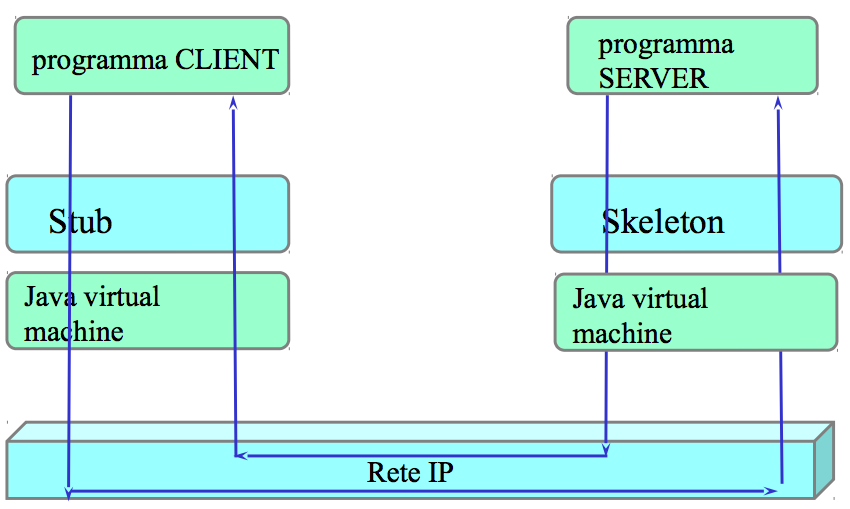
\includegraphics[scale=0.3]{Img/RMIInternal.png}
\centering
\caption{RMI in practice in a nutshell.}
\label{RMIInPracticeHighLevel}
\end{figure}


Il client (la JVM del client) in ``qualche modo" (vedremo dopo ottiene uno stub di un oggetto remoto. Lo stub  \`e un rappresentativo locale di un oggetto remoto (localizzato sul server) che viene utilizzato dal client. Quando il client invoca un messsaggio sullo stub, lo stub ``si rende responsabile" di chiamare il metodo sull'oggetto remoto che si trova sul server.  In particolare, quando \emph{invochiamo un metodo} sullo stub l'oggetto (stub):
\begin{itemize}
\item crea una connessione con la macchina virtuale remota (server) che contiene l'oggetto remoto
\item esegue il marshal dei parametri passati al metodo
\item attende i risultati dell'invocazione del metodo
\item esegue l'unmarshal del valore ritornato
\item ritorna il valore ottenuto
\end{itemize}
Lo stub nasconde sia la serializzazione dei parametri che la comunicazione che avviene a livello di rete.

Il server (la JVM sel server) contiene per ogni oggetto remoto uno skeleton corrispondente. Lo skeleton \`e responsabile della ricezione e dell'invio di messaggi da e al client. Quando riceve un invocazione su uno dei suoi metodi esegue le seguenti azioni:
\begin{itemize}
\item unmarshals (legge) i parametri passati al metodo remoto
\item invoca il metodo sull'oggetto che risiede sul server
\item esegue il marshal del risultato
\item invia il risultato al chiamante
\end{itemize}

Un sequence diagram che descrive il comportament dinamico di un applicazione RMI \`e presentato in Figura~\ref{RMIInPractice}. Il sistema esegue i seguenti passi:

\begin{itemize}
\item il client deve ottenere lo stub dell'oggetto remoto che desidera utilizzare
\item il client invoca un metodo sull'oggetto remoto
\item lo stub chiama il metodo del corrispettivo oggetto sul server,
\item l'oggetto ritorna il valore.
\end{itemize}


\begin{figure}[h]
\centering
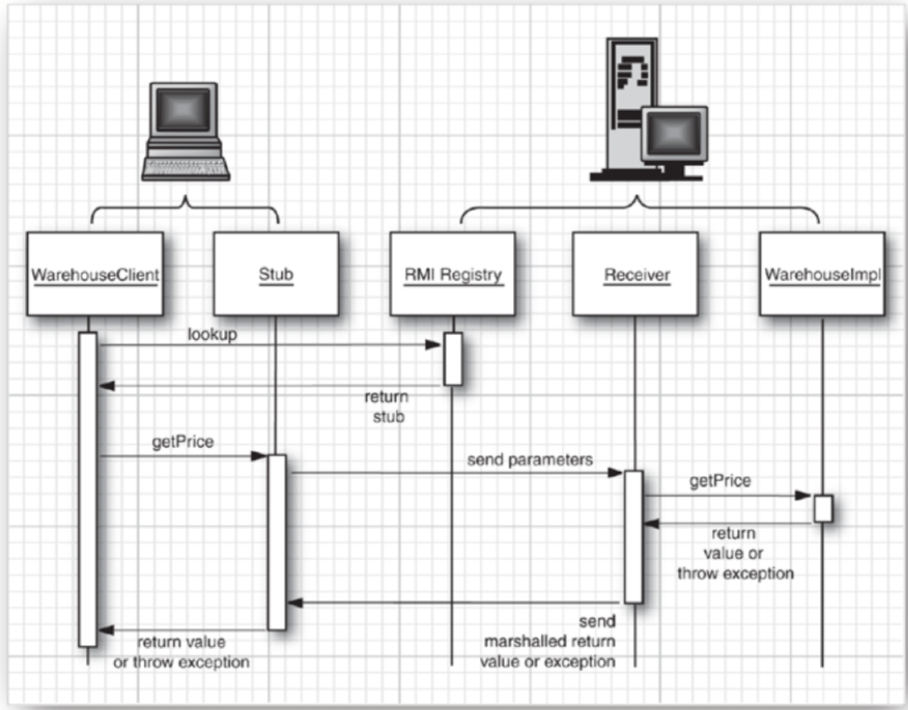
\includegraphics[scale=0.3]{Img/RMI.png}
\centering
\caption{RMI in practice in a nutshell.}
\label{RMIInPractice}
\end{figure}


\subsection{RMI in practice}

\subsubsection{Remote interface, Objects and metods}

\begin{itemize}
\item \emph{remote interface}:  \`e l'interfaccia che dichiara i metodi che possono essere invocati dal client. L'interfaccia deve:
\begin{itemize}
\item deve estendere \texttt{java.rmi.Remote}
\item Ogni metodo dell'interfaccia deve lanciare una eccezione \texttt{java.rmi.RemoteException} in aggiunta alle eccezioni gi\`a lanciate.
\item ogni parametro del metodo dell'interfaccia remota deve:
\begin{itemize}
\item essere serializzabile (questo consente di eseguire marshal and unmarshal) oppure
\item essere un tipo primitivo oppure
\item essere un oggetto remoto
\end{itemize}
\end{itemize}.
\item \emph{remote object}: sono degli oggetti i cui metodi possono essere invocati da una JVM (Java Virtual Machine) differente da quella in cui gli oggetti sono collocati. Gli oggetti remoti sono trattati in maniera differente dagli oggetti normali, quando vengono passati da una JVM ad un altra, viene passato il corrispettivo stub
 \end{itemize}

Immaginiamo di chiamare un metodo di un interfaccia remota che ritorna un oggetto. Due casi sono possibili
\begin{itemize}
\item l'oggetto non \`e remoto. L'oggetto viene serializzato e deserializzato. Il client ottiene una copia dell'oggetto remoto
\item l'oggetto \`e remoto. Viene ottenuto uno stub dell'oggetto remoto. Lo stub \`e un rappresentativo locale o un proxy dell'oggetto remoto (in sostanza un reference remoto).
\item un oggetto remoto deve implementare una interfaccia remota. il client pu\`o invocare sull'oggetto remoto solo i metodi definiti nell'interfaccia.
\end{itemize}


Come menzionato prima ci sono due regole che governano il passaggio di parametri e i valori di ritorno dei metodi:
\begin{itemize}
\item NON Remote Object: sono passati per copia utilizzando la serializzazione di \texttt{Java} 
\item Remote Object: sono passati per reference. Un reference a un remote object \`e uno stub
\end{itemize}

\newpage

\section{Esercizi}
\subsection{Esercizio 1}
\begin{lstlisting}[language=Java,escapechar=|]
import java.io.IOException;
import java.io.InputStreamReader;
import java.io.ObjectOutputStream;
import java.net.Socket;
import java.util.Scanner;

public class Client {
	/**
	 * is the port that the Server uses to wait connections
	 */
	private final static int PORT = 29999;

	/**
	 * starts the Client
	 *
	 * @throws IOException
	 */
	public void startClient() throws IOException {
		/*
		 * creates a new socket that refers to the machine with the specified IP
		 * and PORT 127.0.0.1 refers to your local machine, change this address
		 * if you want to use your program in the network (in case of problems
		 * check your firewall preferences)
		 */
		Socket socket = new Socket("127.0.0.1", PORT);
		System.out.println("Connection Established");
		// creates a new stream that is able to write characters on the socket
		// for more details drag your mouse over the PrintWriter class
		ObjectOutputStream objectOutputStream=new ObjectOutputStream(socket.getOutputStream());
		// creates a new scanner to read input from standard input
		Scanner stdin = new Scanner(new InputStreamReader(System.in));
		while (true) {
			// read the string from the standard input
			String inputLine = stdin.nextLine();
			// sends the read string to the server
			
			Player player=new Player(inputLine);
			objectOutputStream.writeObject(player);
			objectOutputStream.flush();
		}
	}

	public static void main(String[] args) {
		// creates a new Client
		Client client = new Client();
		try {
			// runs the Client
			client.startClient();
		} catch (IOException e) {
			e.printStackTrace();
		}
	}
}
\end{lstlisting}
\begin{lstlisting}[language=Java,escapechar=|]
public class Player implements Serializable{

	private String name;
	
	public Player(String name){
		this.name=name;
	}
	
	public String getName(){
		return this.name;
	}
	@Override
	public String toString() {
		return "Player [name=" + name + "]";
	}
}
\end{lstlisting}
\begin{lstlisting}[language=Java,escapechar=|]
import java.io.IOException;
import java.io.ObjectInputStream;
import java.io.PrintWriter;
import java.net.ServerSocket;
import java.net.Socket;

public class Server {
	/**
	 * is the port that the Server uses to wait connections
	 */
	private final static int PORT = 29999;

	/**
	 * starts the server
	 * 
	 * @throws IOException
	 * @throws ClassNotFoundException 
	 */
	public void startServer() throws IOException, ClassNotFoundException {
		// creates a new Server socket on the specified port
		ServerSocket serverSocket = new ServerSocket(PORT);
		System.out.println("Server socket ready on port: " + PORT);
		// puts the serverSocket in a state where is waiting for client
		// connections
		// the server stops on this instruction until a connection arrives
		Socket socket = serverSocket.accept();
		System.out.println("client connection received");
		// creates a new scanner that is able to read characters from the socket
		// for more detail drag your mouse over the Scanner class
		ObjectInputStream inputStream = new ObjectInputStream(
				socket.getInputStream());
		// creates a new PrintWriter that is able to write characters on the
		// socket
		// for more details drag your mouse over the PrintWriter class
		PrintWriter socketOut = new PrintWriter(socket.getOutputStream());
		boolean end = false;
		// reads and write characters from the socket until the String quit is
		// received
		while (!end) {
			// line contains the String sent by the client
			Player player = (Player) inputStream.readObject();

			System.out.println("SERVER: received the object: "
					+ player.toString());

		}
		System.out.println("Closing the socket");
		// closes the scanner
		inputStream.close();
		// closes the printWriter
		socketOut.close();
		// closes the socket
		socket.close();
		// closes the ServerSocket
		serverSocket.close();
	}

	/**
	 * Runs the Server
	 * 
	 * @param args
	 * @throws ClassNotFoundException 
	 */
	public static void main(String[] main) throws ClassNotFoundException {
		// creates the server
		Server echoServer = new Server();
		try {
			// starts the server
			echoServer.startServer();
		} catch (IOException e) {
			e.printStackTrace();
		}
	}

}
\end{lstlisting}

\subsection{Esercizio 2}
\subsubsection{Oggetto}
\begin{lstlisting}[language=Java,escapechar=|]
public class Oggetto implements Serializable{

    // modificare in private transient String name;
	 // in un secondo momento
	private String name;
	
	public Oggetto(String name){
		this.name=name;
	}
	
	public void changeName(String name){
		this.name=name;
	}

	@Override
	public String toString() {
		return "Oggetto [name=" + name + "]";
	}
}
\end{lstlisting}

\subsubsection{Room}
\begin{lstlisting}[language=Java,escapechar=|]
package server;
import java.rmi.RemoteException;


// implementazione dell'interfaccia remota
public class RMIRoom implements RMIRoomRemote {

	private Oggetto oggetto;
	
	public void printStato() throws RemoteException{
		if(oggetto==null){
			System.out.println("Non sono presenti oggetti");
		}
		else{
			System.out.println(oggetto);
		}
	}
	public void cambiaOggetto(Oggetto oggetto) throws RemoteException{
		this.oggetto=oggetto;
	}
}
\end{lstlisting}

\begin{lstlisting}[language=Java,escapechar=|]
// l'interfaccia remota deve estendere Remote
public interface RMIRoomRemote extends Remote{

	// ogni metodo nell'interfaccia remota deve lanciare l'eccezione
	// RemoteException
	public void printStato() throws RemoteException;
	public void cambiaOggetto(Oggetto oggetto) throws RemoteException;
}
\end{lstlisting}

\subsubsection{Server}
\begin{lstlisting}[language=Java,escapechar=|]
package server;
import java.rmi.AlreadyBoundException;
import java.rmi.RemoteException;
import java.rmi.registry.LocateRegistry;
import java.rmi.registry.Registry;
import java.rmi.server.UnicastRemoteObject;


public class Server {

	private final Registry registry;
	private static final String NAME = "room";
	
	public Server() throws RemoteException, AlreadyBoundException{
		registry = LocateRegistry.createRegistry(1099);
		System.out.println("Constructing server implementation");
		RMIRoom game = new RMIRoom();

		RMIRoomRemote gameRemote = (RMIRoomRemote) UnicastRemoteObject
				.exportObject(game, 0);

		System.out.println("Binding server implementation to registry...");
		registry.bind(NAME, gameRemote);

		System.out.println("Waiting for invocations from clients...");
	
	}

	public static final void main(String[] args) throws RemoteException, AlreadyBoundException{
		new Server();
	}
}
\end{lstlisting}

\subsubsection{Client}
\begin{lstlisting}[language=Java,escapechar=|]
package client;

import java.rmi.NotBoundException;
import java.rmi.RemoteException;
import java.rmi.registry.LocateRegistry;
import java.rmi.registry.Registry;

import server.Oggetto;
import server.RMIRoomRemote;

public class Client {

	private final static String HOST="127.0.0.1";
	private final static int PORT=1099;
	private static final String NAME = "room";
	
	public static void main(String[] args) throws RemoteException, NotBoundException {
		
		Registry registry = LocateRegistry.getRegistry(HOST,PORT);
		RMIRoomRemote game = (RMIRoomRemote) registry.lookup(NAME);
		System.out.println("Invoking remote object...");
		
		game.printStato();
		Oggetto oggetto=new Oggetto("spada");
		game.cambiaOggetto(oggetto);
		game.printStato();
		oggetto.changeName("cubo");
		game.printStato();
		game.cambiaOggetto(oggetto);
		game.printStato();
		
	}
}
\end{lstlisting}

\subsection{Esercizio 3}
\subsubsection{Oggetto}

\begin{lstlisting}[language=Java,escapechar=|]
public class Oggetto extends UnicastRemoteObject implements OggettoRemote{

	private String name;
	
	public Oggetto(String name) throws RemoteException{
		super();
		this.name=name;
	}
	
	public void changeName(String name){
		this.name=name;
	}

	@Override
	public String toString() {
		return "Oggetto [name=" + name + "]";
	}
}
\end{lstlisting}

\begin{lstlisting}[language=Java,escapechar=|]
import java.rmi.Remote;
import java.rmi.RemoteException;

public interface OggettoRemote extends Remote{

	public void changeName(String name)  throws RemoteException;
}
\end{lstlisting}


\subsubsection{RMIRoom}
\begin{lstlisting}[language=Java,escapechar=|]
import java.rmi.RemoteException;


// implementazione dell'interfaccia remota
public class RMIRoom implements RMIRoomRemote {

	private OggettoRemote oggetto;
	
	public RMIRoom() throws RemoteException{
		this.oggetto=new Oggetto("default Oggetto");
		
	}
	
	public OggettoRemote getObject(){
		return this.oggetto;
	}
	
	public void printStato() throws RemoteException{
		if(oggetto==null){
			System.out.println("Non sono presenti oggetti");
		}
		else{
			System.out.println(oggetto);
		}
	}
	public void cambiaOggetto(OggettoRemote oggetto) throws RemoteException{
		this.oggetto=oggetto;
	}
}
\end{lstlisting}

\begin{lstlisting}[language=Java,escapechar=|]
// l'interfaccia remota deve estendere Remote
public interface RMIRoomRemote extends Remote{

	// ogni metodo nell'interfaccia remota deve lanciare l'eccezione
	// RemoteException
	public void printStato() throws RemoteException;
	public void cambiaOggetto(OggettoRemote oggetto) throws RemoteException;
	public OggettoRemote getObject() throws RemoteException;
}
\end{lstlisting}

\begin{lstlisting}[language=Java,escapechar=|]
public class Server {

	private final Registry registry;
	private static final String NAME = "room";

	public Server() throws RemoteException, AlreadyBoundException{
		System.out.println("ciao");
		registry = LocateRegistry.createRegistry(1099);
		System.out.println("Constructing server implementation");
		RMIRoom game = new RMIRoom();
		
		RMIRoomRemote gameStub = (RMIRoomRemote) UnicastRemoteObject
				.exportObject(game, 0);
		

		System.out.println("Binding server implementation to registry...");
		registry.rebind(NAME, gameStub);

		System.out.println("Waiting for invocations from clients...");
	
	}

	public static final void main(String[] args) throws RemoteException,
			AlreadyBoundException {
		new Server();
	}
}
\end{lstlisting}

\begin{lstlisting}[language=Java,escapechar=|]
import java.rmi.NotBoundException;
import java.rmi.RemoteException;
import java.rmi.registry.LocateRegistry;
import java.rmi.registry.Registry;

import server.Oggetto;
import server.OggettoRemote;
import server.RMIRoomRemote;

public class Client {

	private final static String HOST="127.0.0.1";
	private final static int PORT=1099;
	private static final String NAME = "room";
	
	public static void main(String[] args) throws RemoteException, NotBoundException {
		
		
		Registry registry = LocateRegistry.getRegistry(HOST,PORT);
		RMIRoomRemote game = (RMIRoomRemote) registry.lookup(NAME);
		System.out.println("Invoking remote object...");
		
		
		game.printStato();
		OggettoRemote object=game.getObject();
		object.changeName("telefono");
		game.printStato();
		
		OggettoRemote oggetto=new Oggetto("spada");
		game.cambiaOggetto(oggetto);
		game.printStato();
		oggetto.changeName("cubo");
		game.printStato();
		game.cambiaOggetto(oggetto);
		game.printStato();
	}
}
\end{lstlisting}


\subsection{Esercizio 4 Server}
\subsubsection{View}
\begin{lstlisting}[language=Java,escapechar=|]

import game.client.RMIClientRemote;
import game.server.actions.EseguiMossa;
import game.server.model.Mossa;
import game.server.model.Player;

import java.rmi.RemoteException;
import java.rmi.server.UnicastRemoteObject;
import java.util.Observable;

public class ServerRMIGameView extends View implements ServerRMIGameViewRemote {

	private RMIClientRemote client;
	
	protected ServerRMIGameView(RMIClientRemote client) throws RemoteException {
		UnicastRemoteObject.exportObject(this,1099);
		this.client=client;
		
	}
	
	public void performMossa(Mossa mossa, Player player) throws RemoteException{
		this.setChanged();
		this.notifyObservers(new EseguiMossa(mossa, player));
	}

	@Override
	public void update(Observable o, Object arg) {
		System.out.println("SERVER-VIEW-RMI: sending the message " + arg);
		try {
			this.client.print(arg.toString());
		} catch (RemoteException e) {
			// TODO Auto-generated catch block
			e.printStackTrace();
		}
		
	}
}
\end{lstlisting}

\begin{lstlisting}[language=Java,escapechar=|]
import game.server.model.Mossa;
import game.server.model.Player;

import java.rmi.Remote;
import java.rmi.RemoteException;

public interface ServerRMIGameViewRemote extends Remote{

	public void performMossa(Mossa mossa, Player player) throws RemoteException;
}
\end{lstlisting}

\begin{lstlisting}[language=Java,escapechar=|]

import game.client.RMIClientRemote;
import game.server.Server;

import java.rmi.AlreadyBoundException;
import java.rmi.RemoteException;

public class ServerRMIRegistrationView implements ServerRMIRegistrationViewRemote {

	private Server server;

	public ServerRMIRegistrationView(Server server) {
		this.server = server;
	}

	@Override
	public ServerRMIGameViewRemote register(RMIClientRemote client) throws RemoteException, AlreadyBoundException {
		
		ServerRMIGameView view=new ServerRMIGameView(client);
		server.addRMIClient(view);
		return view;
	}
}
\end{lstlisting}

\begin{lstlisting}[language=Java,escapechar=|]
public interface ServerRMIRegistrationViewRemote extends Remote  {
	
	public ServerRMIGameViewRemote register(RMIClientRemote client) throws RemoteException, AlreadyBoundException;

}
\end{lstlisting}

\subsubsection{Server}

\begin{lstlisting}[language=Java,escapechar=|]
import game.server.model.GameState;
import game.server.model.Partita;
import game.server.view.ServerRMIRegistrationView;
import game.server.view.ServerRMIRegistrationViewRemote;
import game.server.view.ServerSocketView;
import game.server.view.View;

import java.io.IOException;
import java.net.ServerSocket;
import java.net.Socket;
import java.rmi.AlreadyBoundException;
import java.rmi.RemoteException;
import java.rmi.registry.LocateRegistry;
import java.rmi.registry.Registry;
import java.rmi.server.UnicastRemoteObject;
import java.util.concurrent.ExecutorService;
import java.util.concurrent.Executors;

/**
 * contains the implementation of the Server class. This server is able to manage multiple clients
 * 
 * @author Claudio Menghi
 * 
 */
public class Server {

	/**
	 * is the port that the Server uses to wait connections
	 */
	private final static int PORT = 29999;
	
	private Partita partita;
	private Controller controller;
	private final Registry registry;
	private static final String NAME = "game";
	
	public Server() throws RemoteException{
		partita=new Partita();
		controller=new Controller(partita);
		registry = LocateRegistry.createRegistry(1099);
		
		
		
	}
	
	public void start() throws AlreadyBoundException, IOException{
		this.startRMI();
		this.startSocket();
	}
	
	private void startRMI() throws RemoteException, AlreadyBoundException{
		System.out.println("Constructing server implementation");
		ServerRMIRegistrationViewRemote game = new ServerRMIRegistrationView(this);

		ServerRMIRegistrationViewRemote gameRemote = (ServerRMIRegistrationViewRemote) UnicastRemoteObject
				.exportObject(game, 0);

		System.out.println("Binding server implementation to registry...");
		registry.bind(NAME, gameRemote);

		System.out.println("Waiting for invocations from clients...");
	}
	
	/**
	 * starts the server
	 * 
	 * @throws IOException
	 */
	private void startSocket() throws IOException {
		/*
		 * ExecutorService represents an asynchronous execution mechanism which
		 * is capable of executing tasks in the background.
		 * Executors.newCachedThreadPool() Creates a thread pool that creates
		 * new threads as needed, but will reuse previously constructed threads
		 * when they are available.
		 */
		ExecutorService executor = Executors.newCachedThreadPool();

		// creates a new Server socket on the specified port
		ServerSocket serverSocket = new ServerSocket(PORT);
		System.out.println("Server socket ready on port: " + PORT);
		System.out.println("Server ready");
		
		while (true) {

			try {
				// puts the serverSocket in a state where is waiting for client
				// connections
				// the server stops on this instruction until a connection
				// arrives
				Socket socket = serverSocket.accept();
				ServerSocketView view=new ServerSocketView(socket);
				this.addClient(view);
				executor.submit(view);
				

			} catch (IOException e) {
				break;
			}
		}
		// shutdown the executor
		executor.shutdown();

		// closes the ServerSocket
		serverSocket.close();
	}
	public synchronized void addRMIClient(View view) throws RemoteException, AlreadyBoundException{
		this.addClient(view);
		ServerRMIRegistrationViewRemote game = new ServerRMIRegistrationView(this);

		ServerRMIRegistrationViewRemote gameRemote = (ServerRMIRegistrationViewRemote) UnicastRemoteObject
				.exportObject(game, 0);
		System.out.println("Binding server implementation to registry...");
		String name = "game";
		registry.rebind(name, gameRemote);

	}

	public synchronized void addClient(View view){
		view.addObserver(controller);
		partita.addObserver(view);
		// Submits a Runnable task for execution
		partita.setGameState(partita.getGameState().nextState());
		if(partita.getGameState().equals(GameState.RUNNING)){
			partita=new Partita();
			controller=new Controller(partita);
		}	
	}
	/**
	 * Runs the Server
	 * 
	 * @param args
	 * @throws AlreadyBoundException 
	 * @throws RemoteException 
	 */
	public static void main(String[] args) throws AlreadyBoundException, RemoteException {
		Server server = new Server();
		// starts the server
		try {
			server.start();
		} catch (IOException e) {
			e.printStackTrace();
		}
	}
}
\end{lstlisting}

\subsubsection{Client}
\begin{lstlisting}[language=Java,escapechar=|]
public class RMIClient extends UnicastRemoteObject implements Serializable, RMIClientRemote {

	/**
	 * 
	 */
	private static final long serialVersionUID = 1L;
	private final static String HOST="127.0.0.1";
	private final static int PORT=1099;
	public RMIClient() throws RemoteException {
		super();
	}

	public static void main(String[] args) throws RemoteException,
			NotBoundException, MalformedURLException, AlreadyBoundException {

		new RMIClient().connect();
	}

	public void connect() throws RemoteException, NotBoundException, MalformedURLException, AlreadyBoundException {
		System.out.println("RMI registry bindings ");

		String name = "game";
		
		Registry registry = LocateRegistry.getRegistry(HOST,PORT);
		ServerRMIRegistrationViewRemote game = (ServerRMIRegistrationViewRemote) registry.lookup(name);
		System.out.println("Invoking remote object...");

		ServerRMIGameViewRemote view=game.register(this);
		while (true) {
			
			Scanner stdin = new Scanner(System.in);

			System.out.println("Insert the player ");
			Player player=new Player(stdin.nextLine());
			
			System.out.println("Insert the mossa ");
			Mossa mossa=Mossa.valueOf(stdin.nextLine());
			
			view.performMossa(mossa, player);
		}

	}

	public void print(String serverMessage) {
		System.out.println("The server says " + serverMessage);
	}
}
\end{lstlisting}

\begin{lstlisting}[language=Java,escapechar=|]
public interface RMIClientRemote extends Remote  {

	public void print(String serverMessage) throws RemoteException;
}
\end{lstlisting}



\clearpage

% ---- Bibliography ----




\addcontentsline{toc}{chapter}{Bibliography}
\bibliographystyle{alpha}
\bibliography{bib}
\nocite{*}


\end{document}

